\documentclass{article}
\usepackage[utf8]{inputenc}
\usepackage[icelandic]{babel}
\usepackage[T1]{fontenc}
\usepackage{graphicx}
\usepackage{mathtools}
\usepackage{amsmath}
\usepackage{amssymb}
\usepackage{minted}


\graphicspath{ {./imgs} }
\title{Verkleg æfing 5 - GHSR}
\author{ttb3@hi.is}
\date{\today}


\begin{document}
\maketitle


\section*{1.}
Verkefnið snérist um að hanna bjöllukerfi fyrir spurningarkeppni og fá þannig að kynnast notkun á vippum og rökrásarhliðum.
Það voru fjórar meginkröfur sem kerfið þurfti að uppfylla:
\begin{enumerate}
    \item Hafa þrjá hnappa, einn fyrir hvorn keppanda og einn fyrir stjórnandan
    \item Þegar keppandi ýtir á hnapp á ljós merkt þeim að lýsast upp og haldast upplýst þangað til stjórnandi núllstillir kerfið
    \item Þegar keppandi ýtir á hnapp, koma í veg fyrir að hinn keppandinn geti kveikt á sínu ljósi fyrr en stjórnandi núllstillir kerfið
    \item Hönnuður ákveður hvað gerist þegar báðir keppendur ýta á sama tíma á hnappinn
\end{enumerate}

\section*{2}
Ég byrjaði á að fylgja kröfunum um kerfið.
\begin{enumerate}
    \item Frekar auðvelt ég set þetta upp í Logisim, þrír takkar og tveir þeirra tengjast ljósum \footnote{Sjá mynd 2.1}
    \item Nú flækist málið aðeins, mig vantar eitthvað sem getur haldið utan um stöðu ljósins eftir að búið er að ýta á takkann og núllstill sjálft sig með öðrum: 
    \begin{enumerate}
        \item Það er mynd af D-Vippu í verkefnalýsingunni þannig ég skelli einni þannig inn í rásina ásamt "klukku" sem tengist í NOT-að merki frá S takkanum.
        \item Til að núllstilla D-Vippurnar tengi ég S takkann í RESET inputið á þeim báðum, nú þegar ég ýti á S takkann núllstillast báðar D-Vippurnar \footnote{Sjá mynd 2.2}
    \end{enumerate} 
    \item Eins og kerfið er núna geta báðir keppendur ýtt hvenær sem er á takkana sína til að kveikja á þeim:
    \begin{enumerate}
        \item Leiðin sem ég notaði til að koma í veg fyrir það var að taka Q' merkið út úr báðum D-Vippunum og senda það inn með and hliði í hina D-Vippuna. 
        Það gerir það að verkum að ef búið er að ýta öðru megin verður Q' false og hin vippan getur ekki uppfært sig. \footnote{Sjá mynd 2.3}
    \end{enumerate}
    \item Síðasta vandamálið hvað á að gera ef báðir keppendur ýta á sama tíma, það er einfallt. Ég, verandi Baldursson, er talsvert hrifnari af stafnum B en stafnum A þannig ef báðir keppndur ýta á sama tíma vinnur B alltaf.
    \item Prófaði það með því að tengja enn einn takka við báðar D-Vippurnar og OR-a það saman við upprunalegu takkanna og viti menn, B vann alltaf.\footnote{Sjá mynd 2.4}
\end{enumerate}

\section{3}
Verkefnið gekk ágætlega, ég þurfti að lesa mér til um D-Vippur og ég er ekki einu sinni viss um að ég skilji þær fullkomlega núna en allavega nógu vel til að byggja þetta kerfi.
Það var skemmtilegt að búa þetta til, alltaf gaman að taka alvöru vandamál og finna lausnir á þeim.

\section*{4}
Myndir:
\begin{center}
    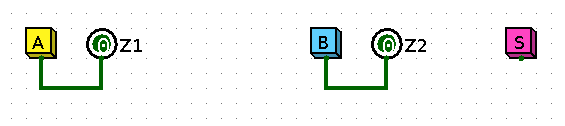
\includegraphics[scale=0.5]{imgs/Screenshot from 2022-03-25 13-50-39.png}
\end{center}
Mynd 2.1
\begin{center}
    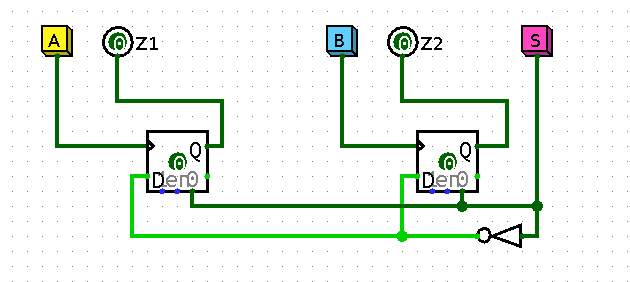
\includegraphics[scale=0.5]{imgs/Screenshot from 2022-03-25 13-57-08.png}
\end{center}
Mynd 2.2
\begin{center}
    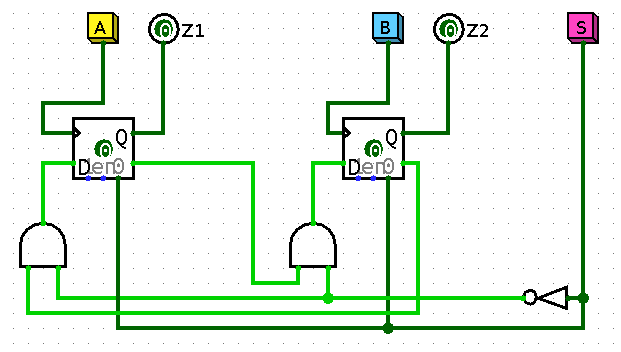
\includegraphics[scale=0.5]{imgs/Screenshot from 2022-03-25 14-00-12.png}
\end{center}
Mynd 2.3
\begin{center}
    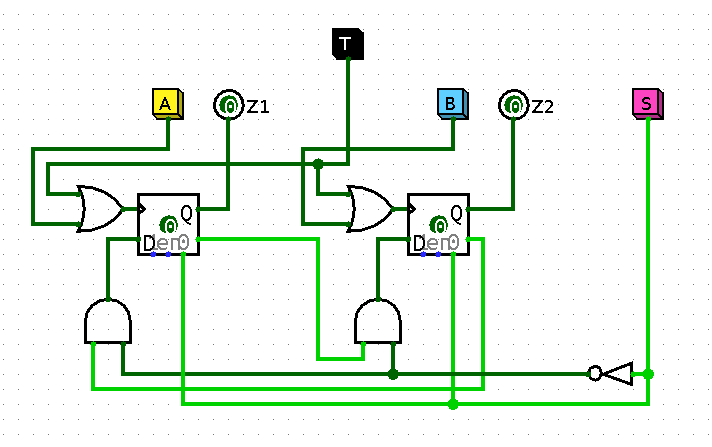
\includegraphics[scale=0.45]{imgs/Screenshot from 2022-03-25 13-00-00.png}
\end{center}
Mynd 2.4

Lokarásin:
\begin{center}
    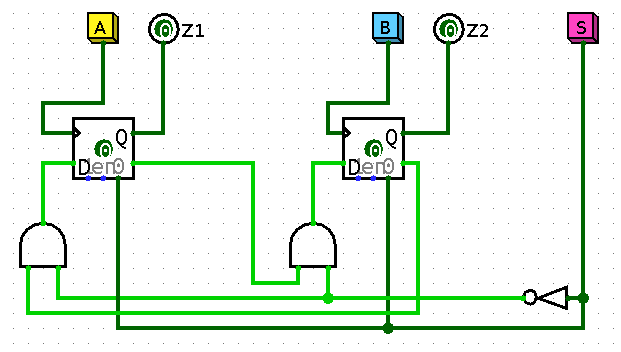
\includegraphics[scale=0.5]{imgs/Screenshot from 2022-03-25 14-00-12.png}
\end{center}

\end{document}